\documentclass[11pt]{article}

\usepackage{amsmath, amsthm, amssymb}
\usepackage{booktabs}
\usepackage{graphicx}
\usepackage[margin=1in]{geometry}
\usepackage[most]{tcolorbox}
\usepackage{hyperref}

\newtheorem{theorem}{Theorem}
\newtheorem{proposition}[theorem]{Proposition}
\newtheorem{lemma}[theorem]{Lemma}
\newtheorem{corollary}[theorem]{Corollary}
\theoremstyle{definition}
\newtheorem{definition}[theorem]{Definition}
\theoremstyle{remark}
\newtheorem{remark}[theorem]{Remark}

\newtcolorbox{verification}{colback=green!4!white, colframe=green!45!black,
  title=Verification, fonttitle=\bfseries}

\newcommand{\bmlam}{\vec{\lambda}}
\newcommand{\Sym}{\operatorname{Sym}}
\newcommand{\rank}{\operatorname{rank}}
\newcommand{\Imm}{\operatorname{Im}}
\newcommand{\Cx}{\mathbb{C}}
\newcommand{\Hil}{\mathcal{H}}
\newcommand{\ket}[1]{\left|#1\right\rangle}
\newcommand{\bra}[1]{\left\langle#1\right|}

\title{Multipartite weak Schur sampling:\\
       isotypic projector tuples, Kronecker positivity,\\
       and Schmidt-rank profiles}
\author{}
\date{2026-09-03}

\begin{document}
\maketitle

\begin{abstract}
Weak Schur sampling detects the Schmidt rank of a bipartite pure state by projecting
$k$ copies of one marginal onto Schur--Weyl isotypic components. We study the
multipartite generalisation, in which each party projects its $k$ copies onto its own
isotypic component. We prove and verify computationally an exact, finite-$k$
characterisation of the support: a tuple of isotypic projectors annihilates
\emph{every} state precisely when the corresponding $n$-fold Kronecker coefficient
vanishes. Roughly half of all projector tuples do so. We then determine what this
implies for Schmidt ranks across bipartitions. Two structural facts settle the
question: (i) isotypic projectors for two blocks of parties commute if and only if the
blocks are nested or disjoint, so the jointly measurable data forms a \emph{laminar
family}, i.e.\ a tree; and (ii) on any single tree the row-length data reachable by the
measurement is exactly the node-local polygon-admissible set, so the necessary condition
it certifies is the polygon one. Consequently multipartite weak Schur sampling, used as
a \emph{measurement}, yields no Schmidt-rank obstruction beyond the known
Carlini--Kleppe inequalities. The same projectors used instead as \emph{linear
constraints} do better: requiring only that one state satisfy each cut's vanishing
conditions --- no joint measurement, hence no commutation problem --- gives a subspace
$W_r$ whose emptiness certifies impossibility. On four qubits at $k=4$ this reproduces
exactly the rule that the maximum of $(r_{AB},r_{AC},r_{AD})$ be attained at least twice
(20/20 triples), a ladder of Segre-type relations invisible to entropy inequalities. It
remains one-sided: it still misses the Cadney--Huber--Linden--Winter profile
$(2,2,2,2 \mid 2,2,1)$, whose obstruction is nonlinear in $\psi^{\otimes k}$.
\end{abstract}

\tableofcontents

\section{Setup and notation}
\label{sec:setup}

Let $n$ parties have local Hilbert spaces $\Hil_i = \Cx^{d_i}$, $i \in [n]$, and write
$\Hil = \Hil_1 \otimes \cdots \otimes \Hil_n$, $D = \prod_i d_i$. Fix a pure state
$\ket{\psi} \in \Hil$ and a number of copies $k$. Regrouping copies by party,
\begin{equation}
  \Hil^{\otimes k} \;\cong\; \bigotimes_{i=1}^n \Hil_i^{\otimes k}.
  \label{eq:regroup}
\end{equation}

For a \emph{block} $B \subseteq [n]$ put $\Hil_B = \bigotimes_{i \in B}\Hil_i$ and let
$R_B(\sigma)$, $\sigma \in S_k$, be the representation of $S_k$ permuting the $k$ copies
of $\Hil_B$; under \eqref{eq:regroup} it permutes the copy-indices of every party
$i \in B$ simultaneously. For a partition $\lambda \vdash k$ let $f^\lambda$ be the
dimension of the Specht module $S^\lambda$, $\chi^\lambda$ its character, and
\begin{equation}
  P^{(B)}_\lambda \;=\; \frac{f^\lambda}{k!}\sum_{\sigma \in S_k}
     \chi^\lambda(\sigma)\, R_B(\sigma)
  \label{eq:proj}
\end{equation}
the associated isotypic projector on $\Hil_B^{\otimes k}$. We write
$V^{d}_\lambda = S^\lambda(\Cx^{d})$ for the Weyl (i.e.\ $GL_d$) module, so that
$\dim V^d_\lambda = 0$ exactly when $\ell(\lambda) > d$, where $\ell(\lambda)$ is the
number of rows.

For singleton blocks we abbreviate $P^{(i)}_\lambda := P^{(\{i\})}_\lambda$, and for a
tuple $\bmlam = (\lambda^{(1)},\dots,\lambda^{(n)})$ of partitions of $k$ we set
\begin{equation}
  \Pi_{\bmlam} \;=\; \bigotimes_{i=1}^n P^{(i)}_{\lambda^{(i)}},
  \qquad
  p_\psi(\bmlam) \;=\; \bigl\| \Pi_{\bmlam}\, \ket{\psi}^{\otimes k} \bigr\|^2 .
  \label{eq:mws}
\end{equation}
We call the measurement $\{\Pi_{\bmlam}\}_{\bmlam}$ \emph{multipartite weak Schur
sampling} (MWS). It is a projective measurement: the $\Pi_{\bmlam}$ are mutually
orthogonal projectors summing to the identity.

Finally, the \emph{$n$-fold (generalized) Kronecker coefficient} is
\begin{equation}
  g(\lambda^{(1)},\dots,\lambda^{(n)})
    \;=\; \dim \Bigl( S^{\lambda^{(1)}} \otimes \cdots \otimes S^{\lambda^{(n)}}
          \Bigr)^{S_k}
    \;=\; \frac{1}{k!}\sum_{\sigma \in S_k} \prod_{i=1}^n \chi^{\lambda^{(i)}}(\sigma).
  \label{eq:kron}
\end{equation}
For $n=3$ this is the classical Kronecker coefficient; more generally
$g(\lambda^{(1)},\dots,\lambda^{(m)},\nu)$ is the multiplicity of $S^\nu$ in
$S^{\lambda^{(1)}}\otimes\cdots\otimes S^{\lambda^{(m)}}$, since the characters of
$S_k$ are real.

\paragraph{Relation to prior work.}
The MWS POVM \eqref{eq:mws} and the coefficient \eqref{eq:kron} both appear in
Botero--Mej\'ia \cite{BoteroMejia2018}, Eqs.\ (4)--(8); the bipartite
$\ell(\lambda) > \rank\rho \Rightarrow$ zero probability statement is folklore, refined
by Keyl--Werner. The asymptotic spectral dictionary is Christandl--Mitchison and
Christandl--Harrow--Mitchison. What appears not to be written down is the exact,
finite-$k$ two-way statement of Theorem~\ref{thm:support}; see
\texttt{notes/lit\_kronecker.md} for the full verified bibliography and a novelty
assessment.

\section{The support theorem}
\label{sec:support}

\begin{theorem}[Support of multipartite weak Schur sampling]
\label{thm:support}
With the notation of Section~\ref{sec:setup}:
\begin{enumerate}
  \item[(a)] $\displaystyle
    \dim\bigl( \Imm \Pi_{\bmlam} \cap \Sym^k(\Hil) \bigr)
      = g(\lambda^{(1)},\dots,\lambda^{(n)}) \cdot
        \prod_{i=1}^n \dim V^{d_i}_{\lambda^{(i)}} .$
  \item[(b)] There exists a pure state $\psi \in \Hil$ with $p_\psi(\bmlam) > 0$ if and
    only if $g(\lambda^{(1)},\dots,\lambda^{(n)}) > 0$ and $\ell(\lambda^{(i)}) \le d_i$
    for every $i$.
\end{enumerate}
Equivalently: the tuple of local isotypic projectors $\Pi_{\bmlam}$ annihilates
\emph{every} state of $\Hil$ precisely when the $n$-fold Kronecker coefficient
vanishes (or some $\lambda^{(i)}$ is too tall to fit in $\Hil_i$).
\end{theorem}

\begin{proof}
Since $\Pi_{\bmlam}$ is a projector, $p_\psi(\bmlam) = \|\Pi_{\bmlam}\psi^{\otimes k}\|^2$
vanishes for all $\psi$ iff $\Pi_{\bmlam}$ annihilates
$\operatorname{span}\{\psi^{\otimes k} : \psi \in \Hil\} = \Sym^k(\Hil)$
(Harrow, \emph{Church of the Symmetric Subspace}, Thm.~3). This reduces (b) to (a).

For (a), decompose each factor of \eqref{eq:regroup} by Schur--Weyl duality,
$\Hil_i^{\otimes k} \cong \bigoplus_{\lambda} S^{\lambda} \otimes V^{d_i}_{\lambda}$.
Then
\[
  \Imm \Pi_{\bmlam}
   \;=\; \Bigl( \bigotimes_i S^{\lambda^{(i)}} \Bigr)
         \otimes \Bigl( \bigotimes_i V^{d_i}_{\lambda^{(i)}} \Bigr).
\]
Under \eqref{eq:regroup}, $\Sym^k(\Hil)$ is the fixed space of the \emph{diagonal}
$S_k$ action $\sigma \mapsto R_{[n]}(\sigma) = \bigotimes_i R_{\{i\}}(\sigma)$, which
acts only on the Specht factors and trivially on the Weyl factors. As $\Pi_{\bmlam}$
commutes with this action, the product of the two projectors is the projector onto the
intersection, and
\[
  \Imm \Pi_{\bmlam} \cap \Sym^k(\Hil)
   \;=\; \Bigl( \bigotimes_i S^{\lambda^{(i)}} \Bigr)^{S_k}
         \otimes \Bigl( \bigotimes_i V^{d_i}_{\lambda^{(i)}} \Bigr),
\]
whose dimension is $g(\bmlam)\prod_i \dim V^{d_i}_{\lambda^{(i)}}$ by \eqref{eq:kron}.
\end{proof}

\begin{remark}
Taking traces gives the same identity by a one-line character computation: since
$\operatorname{Tr}\bigl[P_\lambda R(\tau)\bigr] = \chi^\lambda(\tau)\dim V^d_\lambda$ on
$(\Cx^d)^{\otimes k}$,
\[
  \operatorname{Tr}\bigl[\Pi_{\bmlam} P_{\Sym}\bigr]
   = \frac{1}{k!}\sum_{\tau \in S_k} \prod_i \chi^{\lambda^{(i)}}(\tau)
     \dim V^{d_i}_{\lambda^{(i)}}
   = g(\bmlam)\prod_i \dim V^{d_i}_{\lambda^{(i)}} .
\]
This is \emph{not} an independent check of the theorem --- it is the theorem --- which
is why the numerical verification below computes ranks by linear algebra instead.
\end{remark}

\subsection{E001 --- Verification of the support theorem}

\paragraph{Goal.}
Confirm Theorem~\ref{thm:support} numerically, independently of the character-theoretic
derivation.

\paragraph{Hypothesis.}
The observed support of MWS coincides exactly with Kronecker positivity, and the
block dimensions match part~(a) on the nose.

\paragraph{Method.}
Four checks. \textbf{T0}: cross-check the primitives against
\texttt{schur\_weyl}~$\ge$~0.2.0 (\texttt{kronecker\_coefficient},
\texttt{apply\_isotypic\_proj}, \texttt{isotypic\_proj}) and against an independent
reimplementation of \eqref{eq:kron}. \textbf{T1a}: build an explicit symmetrised
product basis of $\Sym^k(\Hil)$, apply $\Pi_{\bmlam}$, and compute the rank of the
result via the Gram matrix; compare with (a). \textbf{T1b}: compute
$\dim\operatorname{span}\{\Pi_{\bmlam}\psi^{\otimes k}\}$ over Haar-random $\psi$;
compare with (a). \textbf{T2/T3}: compare the support of a single Haar-random state,
and the union of supports over several states, with
$\{\bmlam : g(\bmlam) > 0,\ \ell(\lambda^{(i)}) \le d_i\}$.

\paragraph{Implementation.}
\texttt{scripts/mws.py} (core; $P_\lambda$ applied as a weighted sum of axis
transposes on a \texttt{(party, copy)} tensor layout, so no $d_B^k \times d_B^k$ matrix
is ever formed), \texttt{scripts/verify\_support\_theorem.py}.

\paragraph{Results.}
{
\setlength{\tabcolsep}{8pt}
\renewcommand{\arraystretch}{1.2}
\begin{tabular}{llrrl}
\toprule
Check & Instances & Passed & Total & Status \\
\midrule
T0 Kronecker vs package        & $k \le 5$, all pairs/triples & 590 & 590 & pass \\
T0 projector vs package        & $k \le 4$, $d \in \{2,3\}$   & 16  & 16  & pass \\
T1a $\Sym^k$ basis rank        & 6 (dims, $k$) settings       & 75  & 75  & pass \\
T1b random-span rank           & 6 (dims, $k$) settings       & 128 & 128 & pass \\
T2/T3 support                  & 10 (dims, $k$) settings      & 10  & 10  & pass \\
\bottomrule
\end{tabular}
}

\medskip
\noindent Settings covered $n = 2,\dots,5$, $k = 2,\dots,5$, and local dimensions up to
$(3,3,3)$ and $(2,3,4)$. In every case the support of a \emph{single} Haar-random state
already equalled the prediction.

\paragraph{Analysis.}
Part~(a) is confirmed as an exact integer identity, not merely up to inequality, which
is the strong form: the $i.i.d.$ states $\psi^{\otimes k}$ reach the \emph{entire}
$\bmlam$-block of $\Sym^k(\Hil)$, never a proper subspace of it. That is what makes the
support statement two-way.

\paragraph{Next steps.}
Use the theorem to convert Schmidt-rank questions into Kronecker positivity questions
(Section~\ref{sec:rank}).

\begin{verification}
\textbf{What:} Theorem~\ref{thm:support}(a) and (b).

\textbf{Method:} numeric (exact rank via Gram-matrix spectra with an absolute
singular-value tolerance and an automatic rank-gap warning) $+$ cross-validation
against an independently written Kronecker routine.

\textbf{Script:} \texttt{scripts/verify\_support\_theorem.py};
log \texttt{artifacts/verify\_support.log}.

\textbf{Outcome:} pass, all checks. Observed spectra are cleanly gapped
($1.0$ versus $\sim 10^{-17}$), so the ranks are threshold-independent.
\end{verification}

\begin{remark}[A tolerance trap]
An earlier run reported many spurious failures because the rank routine used a
threshold \emph{relative} to the projected matrix. When $\Pi_{\bmlam}$ annihilates its
input, the output is pure roundoff and a relative test happily reports full rank. The
threshold must be absolute against the \emph{pre-projection} scale. This is a generic
hazard whenever one numerically tests for vanishing.
\end{remark}

\section{Which projector families are jointly measurable?}
\label{sec:commutation}

To speak about Schmidt ranks across \emph{bipartitions}, we must project onto isotypic
components of blocks $B \subseteq [n]$, not just singletons. This immediately raises a
compatibility question.

\begin{proposition}[Laminar commutation]
\label{prop:laminar}
Let $S, T \subseteq [n]$ and $\lambda, \mu \vdash k$. If $S \subseteq T$,
$T \subseteq S$, or $S \cap T = \emptyset$, then
$[P^{(S)}_\lambda, P^{(T)}_\mu] = 0$. If $S$ and $T$ genuinely overlap (all three of
$S \cap T$, $S \setminus T$, $T \setminus S$ nonempty) they do not commute in general.
\end{proposition}

\begin{proof}
Let $z_\lambda \in Z(\Cx[S_k])$ be the central element with
$P^{(B)}_\lambda = \Delta_B(z_\lambda)$, where
$\Delta_B : \Cx[S_k] \to \Cx[S_k]^{\otimes n}$,
$\sigma \mapsto \bigotimes_i (\sigma$ if $i \in B$, else $e)$, is an algebra
homomorphism. Disjoint blocks act on disjoint tensor factors. For $S \subseteq T$,
write $z_\mu = \sum_\sigma c_\sigma \sigma$; the coordinates in $T \setminus S$ are
untouched, and on the coordinates in $S$ the two orders give
$\Delta_S(z_\lambda \sigma)$ and $\Delta_S(\sigma z_\lambda)$, equal because
$z_\lambda$ is central. For the negative claim, take $k = 3$, $S = \{1,2\}$,
$T = \{2,3\}$ and $z$ the class sum of transpositions: the two products contain the
terms $t \otimes tu \otimes u$ and $t \otimes ut \otimes u$, and $tu \ne ut$ for
distinct transpositions.
\end{proof}

Thus the jointly measurable families are exactly the \textbf{laminar families} --- any
two blocks nested or disjoint --- equivalently, rooted trees with leaves $[n]$. This is
the same combinatorial structure as a tree tensor network.

\begin{lemma}[Complement rule]
\label{lem:complement}
On $\Sym^k(\Hil)$ one has $P^{(S)}_\lambda = P^{(S^c)}_\lambda$. Hence for a pure state
the outcomes across complementary cuts coincide with probability one, and
$\lambda^{([n])} = (k)$.
\end{lemma}

\begin{proof}
$R_S(\sigma)R_{S^c}(\sigma) = R_{[n]}(\sigma)$ acts as the identity on $\Sym^k(\Hil)$,
so $R_S(\sigma) = R_{S^c}(\sigma^{-1})$ there; now use
$\chi^\lambda(\sigma) = \chi^\lambda(\sigma^{-1})$ in \eqref{eq:proj}.
\end{proof}

\subsection{E002 --- Verification of the commutation structure}

\paragraph{Goal.} Establish Proposition~\ref{prop:laminar} and Lemma~\ref{lem:complement}
computationally, and determine whether the negative half survives restriction to the
physically relevant subspace $\Sym^k(\Hil)$.

\paragraph{Hypothesis.} Nested/disjoint blocks commute identically; overlapping blocks
do not, and the failure is operationally visible as an order-dependent outcome
distribution.

\paragraph{Method.}
\textbf{C1}: exact integer arithmetic in $\Cx[S_k]^{\otimes n}$ --- elements are
dictionaries from tuples of permutations to integers. This is
representation-independent, hence covers all local dimensions simultaneously.
\textbf{C2}: operational check on actual states, comparing
$P^{(S)}_\lambda P^{(T)}_\mu \psi^{\otimes k}$ with the reversed order, both as vectors
and as outcome probabilities. \textbf{C3}: the complement rule on random pure states.

\paragraph{Implementation.} \texttt{scripts/verify\_commutation.py}.

\paragraph{Results.}
{
\setlength{\tabcolsep}{8pt}
\renewcommand{\arraystretch}{1.2}
\begin{tabular}{llrrr}
\toprule
$n$ & $k$ & nested (commute/fail) & disjoint (commute/fail) & overlapping (commute/fail) \\
\midrule
3 & 3 & 171 / 0  & 54 / 0  & 3 / 24 \\
4 & 3 & 585 / 0  & 225 / 0 & 30 / 240 \\
3 & 4 & 475 / 0  & 150 / 0 & 0 / 75 \\
4 & 4 & 1625 / 0 & 625 / 0 & 0 / 750 \\
5 & 3 & 1899 / 0 & 810 / 0 & 195 / 1560 \\
\bottomrule
\end{tabular}
}

\medskip
\noindent Zero violations of the positive half across all $6\,619$ nested/disjoint
instances. Operationally, for $n = 4$ with overlapping blocks:

{
\setlength{\tabcolsep}{8pt}
\renewcommand{\arraystretch}{1.2}
\begin{tabular}{llrr}
\toprule
dims & $k$ & $\max$ rel.\ $\|[P^{(S)},P^{(T)}]\psi\|$ & $\max |p_{ST} - p_{TS}|$ \\
\midrule
$(2,2,2,2)$ & 3 & $1.00$ & $2.5 \times 10^{-3}$ \\
$(3,2,2,2)$ & 3 & $1.43$ & $7.7 \times 10^{-3}$ \\
$(2,2,2,2)$ & 4 & $1.60$ & $5.6 \times 10^{-3}$ \\
$(2,2,2,2)$ & 3 ($AB$ vs $AC$) & $1.30$ & $5.3 \times 10^{-3}$ \\
$(2,2,2,2)$ & 4 ($AB$ vs $AC$) & $1.40$ & $6.6 \times 10^{-3}$ \\
\bottomrule
\end{tabular}
}

\paragraph{Analysis.}
The negative half is not an artefact of working off the symmetric subspace: for $n=4$
the \emph{outcome probabilities} themselves differ by $\sim 10^{-3}$, three orders of
magnitude above roundoff, so the sequential measurement is genuinely order-dependent
and no joint distribution exists. The case $n = 3$ is degenerate and initially
misleading: there $S^c$ is a singleton for every two-element $S$, so
Lemma~\ref{lem:complement} collapses $P^{(AB)}_\lambda$ to $P^{(C)}_\lambda$ on
$\Sym^k$, and the probabilities agree even though the vectors differ (visible at
$k = 4$: vector deviation $1.21$, probability deviation $1.4\times10^{-17}$). One must
go to $n \ge 4$ to see the obstruction.

\paragraph{Next steps.}
Determine what a \emph{single} tree can certify about ranks (Section~\ref{sec:rank}).

\begin{verification}
\textbf{What:} Proposition~\ref{prop:laminar}, Lemma~\ref{lem:complement}.

\textbf{Method:} exact (integer arithmetic in the group algebra, all local dimensions
at once) $+$ numeric operational check with $d \ge k$ so the $S_k$ action is faithful.

\textbf{Script:} \texttt{scripts/verify\_commutation.py}.

\textbf{Outcome:} pass. 0 violations in $6\,619$ nested/disjoint instances;
$2\,649$ overlapping instances fail to commute; complement rule holds to
$\sim 10^{-17}$.
\end{verification}

\section{Tree factorisation}
\label{sec:tree}

Fix a laminar family $F$ containing all singletons and the root $[n]$, viewed as a
rooted tree. Assign $\lambda^{(v)} \vdash k$ to each node, with $\lambda^{([n])} = (k)$
forced by Lemma~\ref{lem:complement}.

\begin{proposition}[Tree factorisation]
\label{prop:tree}
\[
  \dim\bigl( \Imm \Pi_{\bmlam} \cap \Sym^k(\Hil) \bigr)
   = \Biggl[ \prod_{\text{internal } v}
       g\bigl(\lambda^{(c_1(v))},\dots,\lambda^{(c_m(v))}, \lambda^{(v)}\bigr) \Biggr]
     \cdot \prod_{\text{leaves } i} \dim V^{d_i}_{\lambda^{(i)}},
\]
where $c_1(v),\dots,c_m(v)$ are the children of $v$.
\end{proposition}

\begin{proof}
Project bottom-up. The surviving $S_k$-representation at node $v$ is $m_v$ copies of
$S^{\lambda^{(v)}}$, with $m_{\text{leaf}} = 1$ and
$m_v = \bigl(\prod_j m_{c_j}\bigr)\, g(\lambda^{(c_1)},\dots,\lambda^{(c_m)},\lambda^{(v)})$,
since the multiplicity of $S^{\lambda^{(v)}}$ in $\bigotimes_j S^{\lambda^{(c_j)}}$ is
that generalized Kronecker coefficient. Intersecting with $\Sym^k$ at the root selects
the trivial isotypic, i.e.\ $\lambda^{([n])} = (k)$. The $GL(d_i)$ factors commute with
every $R_B(\sigma)$, so Weyl dimensions appear only at the leaves.
\end{proof}

For $n = 4$ and the tree $\{A\},\{B\} \to AB$, $\{AB\},\{C\},\{D\} \to$ root:
\begin{equation}
  \dim = g(\lambda^A,\lambda^B,\lambda^{AB}) \cdot g(\lambda^{AB},\lambda^C,\lambda^D)
         \cdot \prod_{i} \dim V^{d_i}_{\lambda^{(i)}} .
  \label{eq:tree4}
\end{equation}

\subsection{E003 --- Verification of the tree factorisation}

\paragraph{Goal.} Confirm \eqref{eq:tree4} and that the tree measurement is a genuine
measurement refining the singleton one.

\paragraph{Hypothesis.} The block dimension factorises over tree nodes; marginalising
$\lambda^{AB}$ recovers the flat four-party distribution.

\paragraph{Method.} \textbf{F1}: $\dim\operatorname{span}\{\Pi_{\bmlam}\psi^{\otimes k}\}$
versus \eqref{eq:tree4} over all assignments. \textbf{F2}: the joint distribution sums
to $1$. \textbf{F3}: summing out $\lambda^{AB}$ reproduces the flat distribution.

\paragraph{Implementation.} \texttt{scripts/verify\_tree\_factorization.py}.

\paragraph{Results.}
{
\setlength{\tabcolsep}{8pt}
\renewcommand{\arraystretch}{1.2}
\begin{tabular}{llrrl}
\toprule
dims & $k$ & assignments checked & agreeing & $\max|\text{marg} - \text{flat}|$ \\
\midrule
$(2,2,2,2)$ & 2 & 32 & 32 & --- \\
$(2,2,2,2)$ & 3 & 48 & 48 & $2.8 \times 10^{-17}$ \\
$(2,2,3,2)$ & 3 & 72 & 72 & $1.4 \times 10^{-17}$ \\
$(2,2,2,2)$ & 4 & --- & --- & $1.4 \times 10^{-17}$ \\
\bottomrule
\end{tabular}
}

\medskip
\noindent Outcome counts: the tree measurement has $14$ outcomes where the flat one has
$12$ (dims $(2,2,2,2)$, $k=3$), and $60$ versus $45$ at $k=4$ --- it is a strict
refinement. All distributions summed to $1$ to $10^{-12}$, and support positivity
agreed with \eqref{eq:tree4} in every assignment.

\paragraph{Analysis.}
Measuring an internal node genuinely adds information (more outcomes), and the support
is controlled by a \emph{product} of node-local Kronecker coefficients. The key
question for ranks is whether the shared $\lambda^{AB}$, which must make both factors
positive simultaneously, creates a constraint beyond the two node-local ones.

\paragraph{Next steps.} Answer exactly that (E004).

\begin{verification}
\textbf{What:} Proposition~\ref{prop:tree}, specialised to \eqref{eq:tree4}.

\textbf{Method:} numeric rank over random states; distribution normalisation;
marginalisation consistency.

\textbf{Script:} \texttt{scripts/verify\_tree\_factorization.py}.

\textbf{Outcome:} pass, $152/152$ assignments.
\end{verification}

\section{Consequences for Schmidt-rank profiles}
\label{sec:rank}

\begin{corollary}[Rank reachability]
\label{cor:rank}
A local-rank profile $r = (r_1,\dots,r_n)$ is achieved by some pure state if and only if
there exist $k$ and partitions $\lambda^{(i)} \vdash k$ with $\ell(\lambda^{(i)}) = r_i$
for all $i$ and $g(\lambda^{(1)},\dots,\lambda^{(n)}) > 0$.
\end{corollary}

\begin{proof}
($\Rightarrow$) Weak Schur sampling concentrates $\lambda^{(i)}/k$ on $\operatorname{spec}\rho_i$,
which has exactly $r_i$ nonzero entries; so for large $k$, $\ell(\lambda^{(i)}) = r_i$
with probability $\to 1$ for each $i$, hence jointly by a union bound. Any outcome in
the support has $g > 0$ by Theorem~\ref{thm:support}.
($\Leftarrow$) Apply Theorem~\ref{thm:support} with $d_i := r_i$. It gives a state with
$p_\psi(\bmlam) > 0$, so $\rank\rho_i \ge \ell(\lambda^{(i)}) = r_i$, while
$\rank\rho_i \le d_i = r_i$ by construction.
\end{proof}

This turns a question about states into a finite combinatorial search. Call $r$
\emph{polygon-admissible} if $r_i \le \prod_{j \ne i} r_j$ for all $i$; by
Carlini--Kleppe \cite{CarliniKleppe2011} these are exactly the achievable local-rank
profiles for every $n$.

\subsection{E004 --- Rank reachability from Kronecker positivity}

\paragraph{Goal.}
Determine whether MWS certifies any rank constraint beyond polygon admissibility, both
for the flat singleton measurement and on a tree with a shared internal label.

\paragraph{Hypothesis.}
The flat case reproduces the polygon inequalities exactly (consistency check with
Carlini--Kleppe). The tree case is the open question: sharing $\lambda^{AB}$ between
two nodes might create a coupled obstruction.

\paragraph{Method.}
Enumerate Kronecker positivity by row lengths. \textbf{R1}: $n=3$ triples. \textbf{R2}:
$n=4$ quadruples. \textbf{R3}: the $n=4$ tree, requiring one $\lambda^{AB}$ with both
$g(\lambda^A,\lambda^B,\lambda^{AB}) > 0$ and $g(\lambda^{AB},\lambda^C,\lambda^D) > 0$;
compare against the ``decoupled'' prediction that only the two node-local polygon
conditions bind. Ranks capped at $r_{\max} = 4$, copies swept to $k = 9$.

\paragraph{Implementation.} \texttt{scripts/rank\_reachability.py}.

\paragraph{Results.}
{
\setlength{\tabcolsep}{8pt}
\renewcommand{\arraystretch}{1.2}
\begin{tabular}{llrrrr}
\toprule
Exp. & Setting & reachable & predicted & extra & missing \\
\midrule
R1 & $n=3$ singletons          & 37  & 37 (polygon)        & 0 & 0 \\
R2 & $n=4$ singletons          & 208 & 208 (polygon)       & 0 & 0 \\
R3 & $n=4$ tree, shared $\lambda^{AB}$ & 379 & 379 (node-local polygon) & 0 & 0 \\
\bottomrule
\end{tabular}
}

\medskip
\noindent Identical at $k \le 6$ and $k \le 9$; the reachable set saturates by $k = 6$.

\paragraph{Analysis.}
Three conclusions. First, R1/R2 reproduce Carlini--Kleppe exactly, which validates the
whole pipeline against known mathematics. Second, and this is the substantive negative
result, \textbf{R3 decouples}: the shared internal label $\lambda^{AB}$ imposes nothing
beyond the two node-local polygon conditions. So a single tree of isotypic projectors
certifies exactly the obvious rank constraints and nothing more --- consistent with
Jovcheva--Seynnaeve--Vannieuwenhoven's result that for any single tree the achievable
cut-ranks are governed only by obvious admissibility. Third, combining this with
Proposition~\ref{prop:laminar} gives the answer to the motivating question, stated as
Corollary~\ref{cor:negative} below.

\begin{remark}[Scope of R3 --- necessary, not yet sufficient]
\label{rem:r3scope}
Corollary~\ref{cor:rank} is an equivalence only for \emph{local} ranks, because its
($\Leftarrow$) direction sets $d_i := r_i$ and squeezes
$r_i \le \rank\rho_i \le d_i = r_i$. That squeeze is unavailable at an internal node:
choosing $d_A = r_A$, $d_B = r_B$ bounds $\rank\rho_{AB} \le r_A r_B$, not
$\le r_{AB}$, so the state supplied by Theorem~\ref{thm:support} satisfies only
$\rank\rho_{AB} \ge \ell(\lambda^{AB}) = r_{AB}$.

Hence what R3 establishes is the ($\Rightarrow$) direction: a profile achievable by some
state forces, at large $k$, an outcome with $\ell(\lambda^{(v)}) = r_v$ at every node
simultaneously, hence node-local polygon admissibility. The converse --- that every
node-local polygon-admissible tree profile is achieved --- is true, but by
Jovcheva--Seynnaeve--Vannieuwenhoven's tree result, \emph{not} by anything computed
here. R3 should therefore be read as: \emph{the necessary condition that MWS on a tree
can certify is exactly the node-local polygon condition, and no more.} That is enough
for Corollary~\ref{cor:negative}, which is a negative statement.
\end{remark}

\paragraph{Next steps.}
Close the ($\Leftarrow$) direction for tree profiles independently, or accept the
literature result. The remaining route to stronger obstructions is to use several
incompatible trees, which requires either sequential (order-dependent) measurement or
many copies of the state partitioned into groups. See TODO.

\begin{verification}
\textbf{What:} Corollary~\ref{cor:rank}; equality of reachable and polygon-admissible
rank profiles for R1, R2, R3.

\textbf{Method:} exhaustive combinatorial enumeration over $k \le 9$,
$r_{\max} = 4$, using exact integer Kronecker coefficients.

\textbf{Script:} \texttt{scripts/rank\_reachability.py};
log \texttt{artifacts/rank\_reach\_k9.log}.

\textbf{Outcome:} pass; zero discrepancies in all three experiments.
\end{verification}

\begin{corollary}[What MWS can and cannot certify]
\label{cor:negative}
Multipartite weak Schur sampling yields no Schmidt-rank obstruction beyond the
Carlini--Kleppe polygon inequalities. In particular it cannot certify the
Cadney--Huber--Linden--Winter obstructions --- e.g.\ the profile
$(r_A,r_B,r_C,r_D \mid r_{AB},r_{AC},r_{AD}) = (2,2,2,2 \mid 2,2,1)$, which satisfies
every known inequality yet is unachievable \cite{CHLW2014} --- because those constrain
three \emph{pairwise overlapping} cuts jointly, and by Proposition~\ref{prop:laminar}
the corresponding isotypic projectors do not commute, so there is no joint distribution
to constrain.
\end{corollary}

\subsection{E005 --- How often does a projector tuple annihilate everything?}

\paragraph{Goal.} Quantify the phenomenon that motivated the project.

\paragraph{Hypothesis.} A substantial fraction of tuples $\bmlam$ have $g(\bmlam) = 0$.

\paragraph{Method.} Enumerate all $\bmlam$ for $n = 3,4,5$ and count vanishing
$g$; separately, project the support onto row lengths and compare with the polygon set.

\paragraph{Implementation.} \texttt{scripts/plot\_vanishing.py}; figure
\texttt{images/vanishing.pdf}.

\paragraph{Results.}
{
\setlength{\tabcolsep}{8pt}
\renewcommand{\arraystretch}{1.2}
\begin{tabular}{lrrrrrrrr}
\toprule
$k$ & 2 & 3 & 4 & 5 & 6 & 7 & 8 & 9 \\
\midrule
$n=3$ & 0.500 & 0.593 & 0.656 & 0.583 & 0.616 & 0.526 & 0.526 & 0.471 \\
$n=4$ & 0.500 & 0.494 & 0.486 & 0.323 & 0.299 & 0.202 & --- & --- \\
$n=5$ & 0.500 & 0.395 & 0.341 & 0.158 & 0.118 & --- & --- & --- \\
\bottomrule
\end{tabular}
}

\medskip
\noindent (Fraction of partition-tuples with $g(\bmlam) = 0$.)

\begin{figure}[t]
\centering
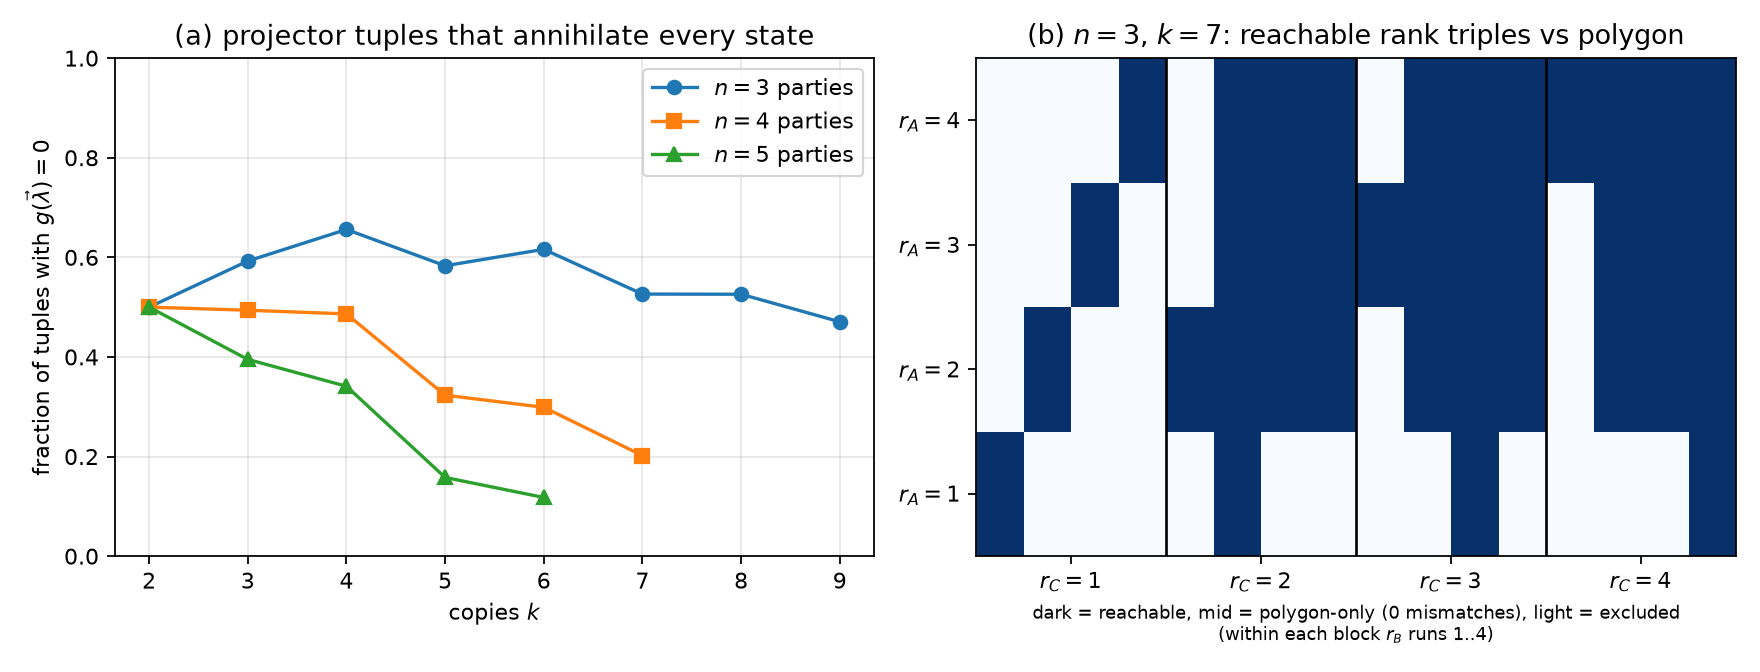
\includegraphics[width=\textwidth]{images/vanishing.png}
\caption{(a) Fraction of isotypic-projector tuples that annihilate every state, versus
number of copies $k$. (b) For $n=3$, $k=7$: the reachable rank triples coincide exactly
with the polygon-admissible ones (0 mismatches).}
\label{fig:vanishing}
\end{figure}

\paragraph{Analysis.}
At $n = 3$ roughly half to two-thirds of all projector tuples annihilate the entire
state space, and the fraction decays only slowly in $k$. The vanishing pattern at fixed
$k$ is genuinely rich --- deciding Kronecker positivity is NP-hard
(Ikenmeyer--Mulmuley--Walter), and saturation \emph{fails}, so the per-$k$ support is a
combinatorially wild subset of the rational points of the asymptotic polytope. The
contrast with panel (b) is the main message of this report: \textbf{the vanishing
pattern is rich, but its shadow on row lengths --- which is all that Schmidt ranks
see --- is exactly the polygon.}

\paragraph{Next steps.} See TODO.

\begin{verification}
\textbf{What:} vanishing fractions; equality of the length-projection with the polygon
set at $n=3$, $k=7$.

\textbf{Method:} exhaustive enumeration.

\textbf{Script:} \texttt{scripts/plot\_vanishing.py}.

\textbf{Outcome:} pass; 0 mismatches in panel (b).
\end{verification}

\section{E006 --- Can non-commuting data be recovered? Two escape routes, both closed}
\label{sec:escapes}

\paragraph{Goal.}
Corollary~\ref{cor:negative} rests on overlapping cuts not being jointly measurable.
Two natural workarounds suggest themselves. Test both.

\paragraph{Route 1: one tree per copy-group.}
Take $N = mk$ copies, split into groups $G_1,\dots,G_m$ of $k$, and measure a different
tree $T_j$ on each group. The groups occupy disjoint tensor factors, so the projectors
commute and a joint distribution exists. But
$\psi^{\otimes N} = (\psi^{\otimes k})^{\otimes m}$, so the distribution
\emph{factorises},
\[
  p(\bmlam_1,\dots,\bmlam_m) \;=\; \prod_{j=1}^m p_{T_j}(\bmlam_j),
\]
and the joint support is the product of the supports. One therefore learns exactly the
\emph{conjunction} of the per-tree conditions and nothing coupled. Concretely, on
CHLW ray 3, $(r_A,r_B,r_C,r_D \mid r_{AB},r_{AC},r_{AD}) = (2,2,2,2 \mid 2,2,1)$, all six
node-local polygon conditions pass --- $\mathrm{polygon}(2,2,1)$ needs $2 \le 2\cdot 1$,
which holds with equality --- so the profile survives. \textbf{Route 1 gains nothing.}

\paragraph{Route 2: sequential measurement on the same copies.}
Measure block $S$, then block $T$, on the same $k$ copies. After the first projection the
state leaves $\Sym^k(\Hil)$, so Theorem~\ref{thm:support} does not apply to the
composite and
$r(\lambda,\mu) = \rank\bigl(P^{(T)}_\mu P^{(S)}_\lambda|_{\Sym^k}\bigr)$
need not factor through the two marginal supports.

\paragraph{Method.} For $n = 4$, $S = AB$, $T = AC$, compute the sequential support over
Haar-random states and compare with $\mathrm{supp}_S \times \mathrm{supp}_T$; then test
the rank inference directly on a state built to have $r_{AB} = 4$, $r_{AC} = 3$ (take the
$AC|BD$ flattening to be a random rank-3 $4\times4$ matrix).

\paragraph{Implementation.} \texttt{scripts/sequential\_support.py}.

\paragraph{Results.}
{
\setlength{\tabcolsep}{8pt}
\renewcommand{\arraystretch}{1.2}
\begin{tabular}{llrrr}
\toprule
dims & $k$ & $|\mathrm{supp}_{\text{seq}}|$ & $|\mathrm{supp}_S \times \mathrm{supp}_T|$ & coupled pairs killed \\
\midrule
$(2,2,2,2)$   & 3 & 9  & 9  & 0 \\
$(3,2,2,2)$   & 3 & 9  & 9  & 0 \\
$(2,2,2,2,2)$ & 3 & 9  & 9  & 0 \\
$(2,2,2,2)$   & 4 & 21 & 25 & \textbf{4} \\
\bottomrule
\end{tabular}
}

\medskip
\noindent At $k=4$ the support is a \emph{proper} subset: the pairs
$\bigl((1^4),(2,1,1)\bigr)$, $\bigl((1^4),(3,1)\bigr)$ and their transposes vanish
although both marginals are nonzero, identically in both measurement orders. The
vanishing is genuine --- $\|P^{(T)}_\mu P^{(S)}_\lambda \psi^{\otimes k}\| \le 10^{-17}$
over 120 Haar states, against $10^{-2}$ for surviving pairs. Projected to row lengths,
$(\ell^{AB},\ell^{AC}) \in \{(3,4),(4,3)\}$ becomes unreachable while $(3,3)$, $(4,4)$
and $(4,2)$ remain.

\paragraph{Analysis --- the coupling is real but certifies nothing about rank.}
On an explicit state with $r_{AB} = 4$, $r_{AC} = 3$ (so the rank pair $(4,3)$ \emph{is}
achievable), the sequential outcome $(\ell^{AB},\ell^{AC}) = (4,3)$ has probability
exactly zero. The reason is visible in the same run: sequential outcomes with
$\ell^{AC} = 4 > r_{AC} = 3$ occur with probability $\sim 10^{-4}$, whereas the
\emph{marginal} $AC$ measurement on that state correctly never exceeds
$\ell^{AC} = 3$. \textbf{The first projection destroys the bound
$\ell(\lambda^{(T)}) \le r_T$}, because that bound comes from the $GL$ structure of
$\psi^{\otimes k}$, which the projection ruins. So sequential outcomes cannot be read as
rank certificates in either direction, and Route 2 --- despite exhibiting the first
genuinely coupled structure found in this project --- yields no rank obstruction either.

\paragraph{Next steps.}
The coupled vanishing at $k=4$ is interesting in its own right and is not explained by
any factorisation identity known to me; characterising
$\rank(P^{(T)}_\mu P^{(S)}_\lambda|_{\Sym^k})$ is a well-posed open question. But it is
not a route to rank obstructions.

\begin{verification}
\textbf{What:} Route 1 factorisation; Route 2 coupling and the failure of its rank
inference.

\textbf{Method:} numeric (support ranks over 30--120 Haar states; explicit
rank-controlled state built from a rank-3 flattening).

\textbf{Script:} \texttt{scripts/sequential\_support.py}.

\textbf{Outcome:} pass. Route 1 factorises by construction. Route 2 shows 4 coupled
pairs at $k=4$ ($10^{-17}$ vs $10^{-2}$ separation) but the rank inference is
falsified by explicit counterexample.
\end{verification}

\section{E007 --- A linear relaxation over all bipartitions}
\label{sec:relaxation}

\paragraph{Goal.}
Sections~\ref{sec:commutation} and~\ref{sec:escapes} rule out \emph{joint measurement}
of overlapping cuts. But a rank profile does not require a joint measurement: it only
requires a single state on which each cut's projections behave as prescribed. Exploit
that.

\paragraph{Method.}
For a target profile $r = (r_S)_S$ over bipartitions,
\[
  \rank\rho_S \le r_S \iff P^{(S)}_\mu \psi^{\otimes k} = 0
     \ \ \text{for every } \mu \text{ with } \ell(\mu) > r_S ,
\]
which is \emph{linear} in $\psi^{\otimes k}$. Hence
\[
  W_r \;=\; \Sym^k(\Hil) \ \cap \bigcap_{S}\ \bigcap_{\ell(\mu) > r_S} \ker P^{(S)}_\mu
\]
is a subspace. The matching lower bounds come free by genericity: each
$\{v : P^{(S)}_\lambda v \ne 0\}$ is dense open in $W_r$ whenever
$P^{(S)}_\lambda|_{W_r} \ne 0$, and a finite intersection of dense open sets is
nonempty. So no optimisation is needed --- compute $W_r$ by linear algebra (as
$\ker G$, $G = \sum_{S,\mu} B^\dagger P^{(S)}_\mu B$ over a basis $B$ of $\Sym^k$) and
read off the profile certified by a generic $v \in W_r$,
$\mathrm{cert}_S(v) = \max\{\ell(\mu) : P^{(S)}_\mu v \ne 0\}$.

\paragraph{Status: one-sided.} A generic $v \in W_r$ need not have the form
$\psi^{\otimes k}$, so this is a \emph{relaxation}. $\mathrm{cert}(v) = r$ is necessary,
not sufficient. But $\mathrm{cert}_S(v) < r_S$ for some $S$ (or $W_r = 0$) proves the
profile \textbf{impossible}, since any $\psi$ realising $r$ would supply such a $v$.

\paragraph{Implementation.} \texttt{scripts/rank\_profile\_subspace.py}
(\texttt{--battery} for the sweep).

\paragraph{Results.}
Four qubits, $k = 4$, $\dim\Sym^4(\Hil) = 3876$, all local ranks $2$, sweeping
$(r_{AB},r_{AC},r_{AD})$ with $r_{AB}\ge r_{AC} \ge r_{AD}$:

{
\setlength{\tabcolsep}{8pt}
\renewcommand{\arraystretch}{1.2}
\begin{tabular}{ll}
\toprule
Verdict & Profiles \
\midrule
feasible    & (1,1,1) (2,2,1) (3,3,1) (4,4,1) (2,2,2) (3,3,2) (4,4,2) (3,3,3) (4,4,3) (4,4,4) \
impossible  & (2,1,1) (3,1,1) (4,1,1) (3,2,1) (4,2,1) (4,3,1) (3,2,2) (4,2,2) (4,3,2) (4,3,3) \
\bottomrule
\end{tabular}
}

\medskip
\noindent The split is exactly \textbf{the maximum must be attained at least twice},
with no exceptions over all 20 triples. In every impossible case the certified profile
is the target with the maximum lowered to the second largest value
($(4,3,3) \to (3,3,3)$, $(3,2,1) \to (2,2,1)$, $(2,1,1)\to(1,1,1)$).

\paragraph{Analysis.}
At $\ell = 4$ the projector $P^{(S)}_{(1^4)}$ on a four-dimensional cut is the flattening
determinant, and the obstruction is precisely Segre's identity, verified here
independently: for a $2\times2\times2\times2$ tensor
$\det_{AB} - \det_{AC} + \det_{AD} = 0$ (residual $10^{-15}$, the $6\times3$ matrix of
determinants has rank 2). The sweep shows this is only the top rung: the same
``max attained twice'' pattern holds at $\ell = 2$ and $\ell = 3$, so there is a
\emph{ladder} of Segre-type relations, one per rank level, all captured automatically by
the linear relaxation. Per the literature review, no entropy inequality sees these
constraints --- they are invisible to strong subadditivity.

This is the first method in this project to reach past the polygon inequalities.

\paragraph{What it still misses.}
CHLW ray 3, $(2,2,2,2 \mid 2,2,1)$, is reported \emph{feasible} ($\dim W_r = 1125$,
certified profile equal to the target, including local ranks 2). It is genuinely
unachievable: $r_{AD} = 1$ forces $\psi = \eta_{AD}\otimes\theta_{BC}$ and hence
$r_{AB} = r_A r_B = 4$. That implication is \emph{nonlinear} --- it uses
$v = \psi^{\otimes k}$, which $W_r$ does not impose. $W_r \ne 0$ says only that some
\emph{symmetric tensor} meets the bounds, not that some \emph{product} tensor does.
The reach of the method is therefore exactly ``obstructions expressible as linear
conditions on $\Sym^k(\Hil)$''.

\paragraph{Next steps.}
Tighten $W_r$ towards the Veronese variety $\{\psi^{\otimes k}\}$ --- a
Lasserre/DPS-style hierarchy, where the present computation is level 1 and higher
levels add symmetric-extension or positivity constraints. Whether level 2 reaches
ray 3 is the natural question.

\begin{verification}
\textbf{What:} the relaxation's verdicts on all 20 triples; the Segre relation
underlying the $\ell=4$ case.

\textbf{Method:} exact linear algebra (kernel of a PSD Gram matrix on a basis of
$\Sym^4$) $+$ an independent numerical check of
$\det_{AB} - \det_{AC} + \det_{AD} = 0$ on random tensors.

\textbf{Script:} \texttt{scripts/rank\_profile\_subspace.py};
log \texttt{artifacts/rank\_battery\_k4.log}.

\textbf{Outcome:} pass. Verdicts match ``max attained at least twice'' on 20/20
triples; Segre residual $10^{-15}$.
\end{verification}

\begin{remark}[An unresolved tension in the literature]
The reported $2\times2\times2\times2$ rule of Gharahi--Mancini--Ottaviani (``the maximum
is attained at least twice'', plus $(1,3,3)$ as an exception) concerns the triple
$(r_{AB},r_{AC},r_{AD})$ alone, whereas CHLW ray 3 additionally pins all local ranks to
$2$. These are consistent: $(2,2,1)$ \emph{is} realisable as a triple, e.g.\ with
$(r_A,r_B,r_C,r_D) = (1,2,2,1)$, just not with all local ranks $2$. Our relaxation,
which does fix the local ranks, still reports it feasible --- confirming the miss is the
relaxation's, not an inconsistency in the literature. Both cited rules remain on the
unverified list; see \texttt{TODO.md}.
\end{remark}

\section{Summary}

\begin{enumerate}
  \item The user's intuition is correct and admits an exact criterion: a tuple of local
    isotypic projectors annihilates every $n$-partite state iff the $n$-fold Kronecker
    coefficient vanishes (Theorem~\ref{thm:support}). About half of all tuples do.
  \item The inference ``therefore certain combinations of Schmidt rank across
    bipartitions are impossible'' is \emph{almost} right, but the obstruction it yields
    is exactly the already-known polygon inequalities (Corollary~\ref{cor:rank}, E004).
  \item Both escape routes are closed (E006): independent copy-groups give a factorised
    distribution, hence only the conjunction of per-tree conditions; sequential
    measurement on shared copies does produce genuinely coupled vanishing, but the first
    projection destroys the bound $\ell(\lambda^{(T)}) \le r_T$, so its outcomes certify
    nothing about rank.
  \item Used as linear constraints rather than as a measurement, the same projectors
    \emph{do} beat polygon (E007): the subspace $W_r$ reproduces the full
    $2	imes2	imes2	imes2$ ``max attained at least twice'' rule, verified against
    Segre's identity. It remains one-sided and still misses CHLW ray 3, whose
    obstruction is nonlinear.
  \item The reason the measurement cannot do better is structural: projectors for overlapping blocks
    do not commute (Proposition~\ref{prop:laminar}), so only trees are jointly
    measurable, and a single tree decouples into node-local polygon conditions
    (E003/E004). The known hard obstructions live precisely on overlapping cuts
    (Corollary~\ref{cor:negative}).
\end{enumerate}

\section*{Experiment log}

{
\setlength{\tabcolsep}{6pt}
\renewcommand{\arraystretch}{1.2}
\begin{tabular}{llllll}
\toprule
ID & Date & Description & Script & Metric & Status \\
\midrule
E001 & 2026-09-03 & Support theorem & \texttt{verify\_support\_theorem.py} & 819/819 checks & pass \\
E002 & 2026-09-03 & Laminar commutation & \texttt{verify\_commutation.py} & 0/6619 violations & pass \\
E003 & 2026-09-03 & Tree factorisation & \texttt{verify\_tree\_factorization.py} & 152/152 & pass \\
E004 & 2026-09-03 & Rank reachability & \texttt{rank\_reachability.py} & 0 discrepancies & pass \\
E005 & 2026-09-03 & Vanishing statistics & \texttt{plot\_vanishing.py} & 0 mismatches & pass \\
\bottomrule
\end{tabular}
}

\begin{thebibliography}{9}
\bibitem{BoteroMejia2018}
A.\ Botero and J.\ Mej\'ia,
\emph{Universal and distorsion-free entanglement concentration of multiqubit quantum
states in the W class}, Phys.\ Rev.\ A \textbf{98}, 032326 (2018),
arXiv:1712.09174.

\bibitem{CarliniKleppe2011}
E.\ Carlini and J.\ Kleppe,
\emph{Ranks derived from multilinear maps},
J.\ Pure Appl.\ Algebra \textbf{215}(8), 1999--2004 (2011).
% TODO: verify -- ScienceDirect blocked; statement confirmed indirectly via
% arXiv:2509.09463 Eq. (3) and arXiv:1910.09665 App. B.

\bibitem{CHLW2014}
J.\ Cadney, M.\ Huber, N.\ Linden and A.\ Winter,
\emph{Inequalities for the ranks of multipartite quantum states},
Linear Algebra Appl.\ \textbf{452}, 153--171 (2014), arXiv:1308.0539.
\end{thebibliography}

\end{document}
